\documentclass[10pt]{article}
\usepackage{tikz}
\usetikzlibrary{shapes.misc}
\usepackage[margin=0cm]{geometry}
\pagestyle{empty}
\tikzstyle{every node}=[cross out, draw, red]

\begin{document}

\vspace*{\fill}
\begin{center}
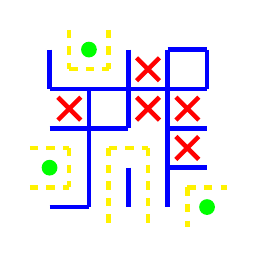
\begin{tikzpicture}[x=0.5cm, y=-0.5cm, ultra thick, blue]
% Walls
    \draw (3,0) -- (4,0);
    \draw (0,1) -- (4,1);
    \draw (0,2) -- (2,2);
    \draw (3,2) -- (4,2);
    \draw (3,3) -- (4,3);
    \draw (0,4) -- (1,4);
    \draw (0,0) -- (0,1);
    \draw (1,1) -- (1,4);
    \draw (2,0) -- (2,2);
    \draw (2,3) -- (2,4);
    \draw (3,0) -- (3,4);
    \draw (4,0) -- (4,1);
% Pillars
    \fill[green] (1,0) circle(0.2);
    \fill[green] (0,3) circle(0.2);
    \fill[green] (4,4) circle(0.2);
% Inner points in accessible cul-de-sacs
    \node at (2.5,0.5) {};
    \node at (0.5,1.5) {};
    \node at (2.5,1.5) {};
    \node at (3.5,1.5) {};
    \node at (3.5,2.5) {};
% Entry-exit paths without intersections
    \draw[dashed, yellow] (0.5,0.5) -- (1.5,0.5);
    \draw[dashed, yellow] (-0.5,2.5) -- (0.5,2.5);
    \draw[dashed, yellow] (1.5,2.5) -- (2.5,2.5);
    \draw[dashed, yellow] (-0.5,3.5) -- (0.5,3.5);
    \draw[dashed, yellow] (3.5,3.5) -- (4.5,3.5);
    \draw[dashed, yellow] (0.5,-0.5) -- (0.5,0.5);
    \draw[dashed, yellow] (0.5,2.5) -- (0.5,3.5);
    \draw[dashed, yellow] (1.5,-0.5) -- (1.5,0.5);
    \draw[dashed, yellow] (1.5,2.5) -- (1.5,4.5);
    \draw[dashed, yellow] (2.5,2.5) -- (2.5,4.5);
    \draw[dashed, yellow] (3.5,3.5) -- (3.5,4.5);
\end{tikzpicture}
\end{center}
\vspace*{\fill}

\end{document}
